% ==============================================================================
% CHAPITRE 5 : TABLEAU DE BORD D'INVESTIGATION (NEXT.JS)
% ==============================================================================

\chapter{Tableau de Bord d'Investigation (Next.js)}
\label{ch:dashboard}

\section{Objectifs et architecture de l'interface utilisateur}

Pour permettre aux analystes de conformité bancaire (\textit{Compliance Officers}) d'exploiter efficacement les alertes produites par le moteur Spark, nous avons développé une application web dédiée à l'investigation médico-légale. L'objectif ergonomique est de fournir une interface sobre et rapide, permettant de comprendre la structure d'un cycle frauduleux en quelques secondes sans être distrait par des animations superflues.

L'application est construite avec **Next.js 14** (App Router), **TypeScript**, **Tailwind CSS** et la bibliothèque de composants **shadcn/ui** :
\begin{itemize}
    \item \textbf{Routes d'API serveur (\texttt{src/app/api/}) :} Des endpoints modulaires (\texttt{/api/alerts}, \texttt{/api/metrics}, \texttt{/api/health}) interrogent directement les tables Delta Lake ou consomment le flux Kafka pour restituer les données en temps réel ;
    \item \textbf{Composants interactifs réactifs :} Maintien d'un état local synchronisé permettant le tri instantané et l'inspection détaillée des transactions.
\end{itemize}

Comme le montre la vue d'ensemble (Figure~\ref{fig:dash_overview}), l'interface restitue les indicateurs de débit, le volume cumulé de transactions traitées et le statut opérationnel de la détection en direct.

\begin{figure}[htbp]
    \centering
    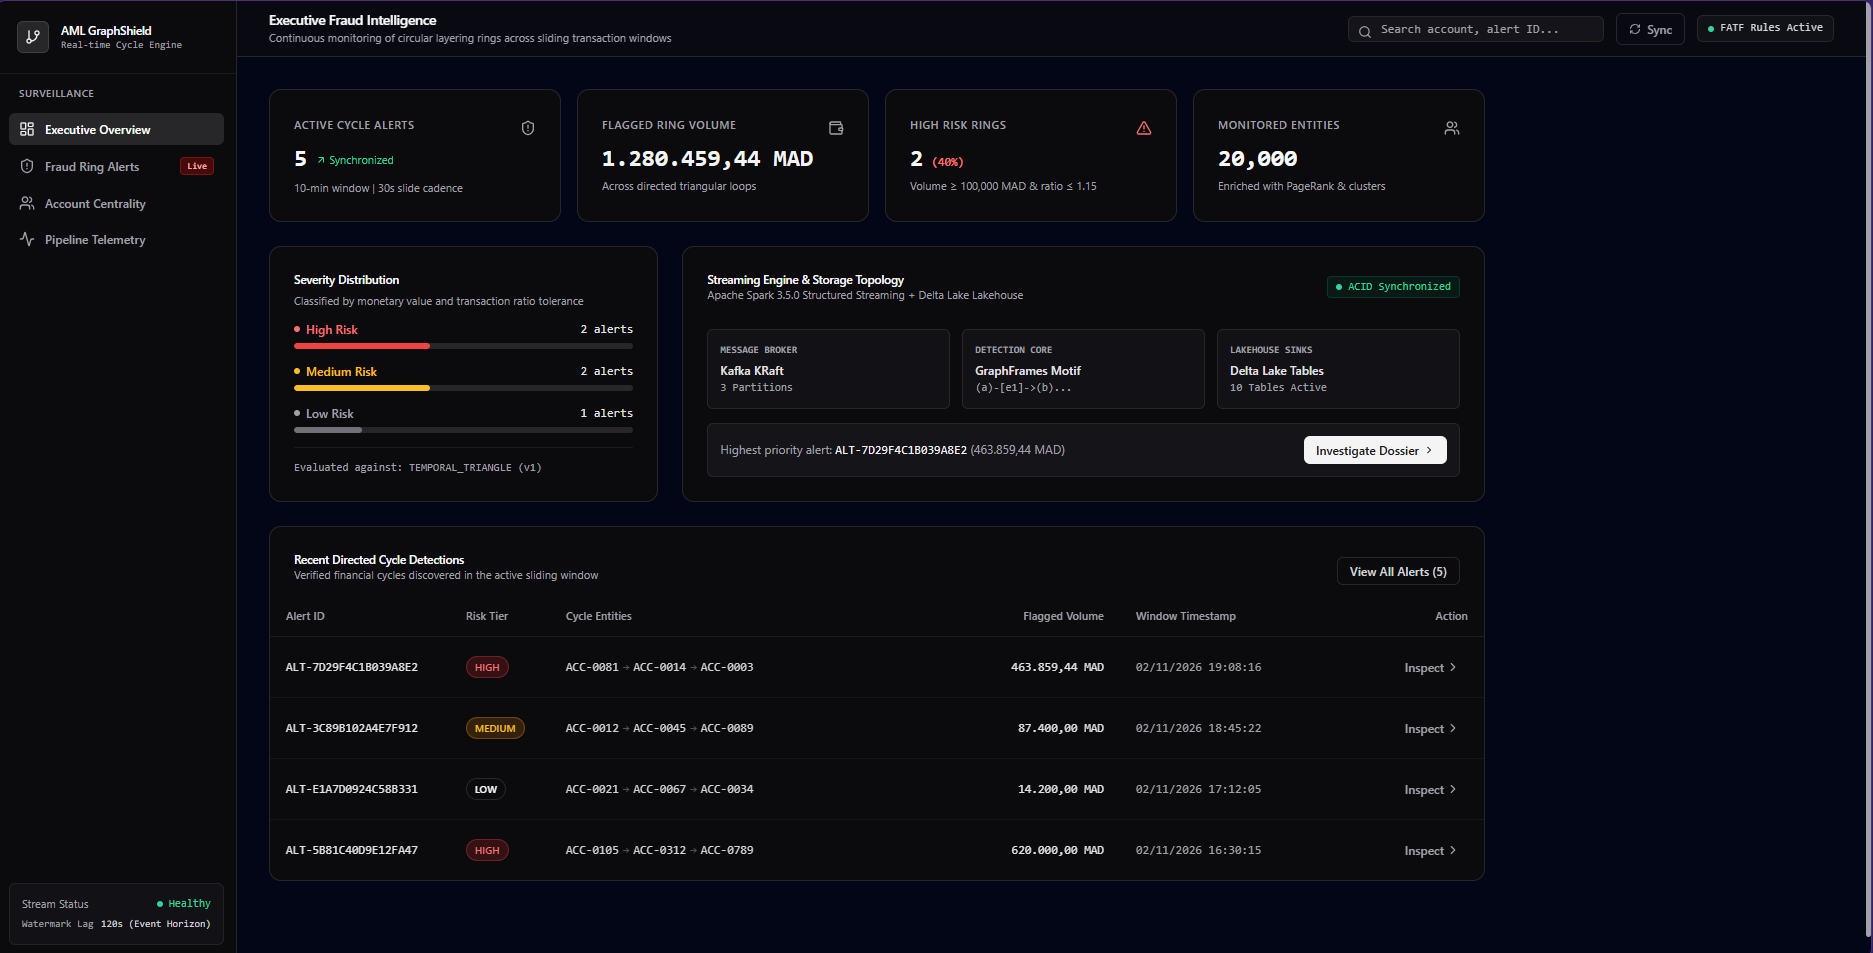
\includegraphics[width=0.92\linewidth]{figures/fig_screenshot_dashboard_overview.png}
    \caption{Tableau de bord d'investigation AML (Next.js 14) : vue exécutive et indicateurs de pilotage (KPIs)}
    \label{fig:dash_overview}
\end{figure}

\section{Moteur de rendu vectoriel (Directed Canvas Graph)}

Le cœur visuel de l'outil est le composant interactif \textbf{DirectedCanvasGraph} (\texttt{network-graph.tsx}). Il génère un canevas vectoriel SVG dynamique qui positionne les comptes du cycle et matérialise les flux :
\begin{itemize}
    \item \textbf{Positionnement trigonométrique :} Les sommets du cycle d'ordre $k=3$ sont positionnés aux sommets d'un triangle équilatéral équi-angulaire centré dans le canevas ;
    \item \textbf{Arêtes courbes et flèches de direction :} Chaque transfert est représenté par un arc orienté avec marqueur fléché indiquant clairement le sens de circulation des fonds ;
    \item \textbf{Affichage des montants et délais :} Chaque arc porte un badge lisible indiquant le montant en Dirhams marocains (\texttt{MAD}) et l'écart temporel $\Delta t$ séparant les virements consécutifs ;
    \item \textbf{Inspecteur de détails au clic :} Le clic sur un nœud ou une arête ouvre un panneau contextuel affichant l'identifiant brut de la transaction, l'horodatage précis et le hash de charge utile.
\end{itemize}

La Figure~\ref{fig:dash_graph} illustre le rendu vectoriel d'un cycle fermé détecté, mettant en évidence les flux d'intermédiation et la conservation quasi-totale des montants.

\begin{figure}[htbp]
    \centering
    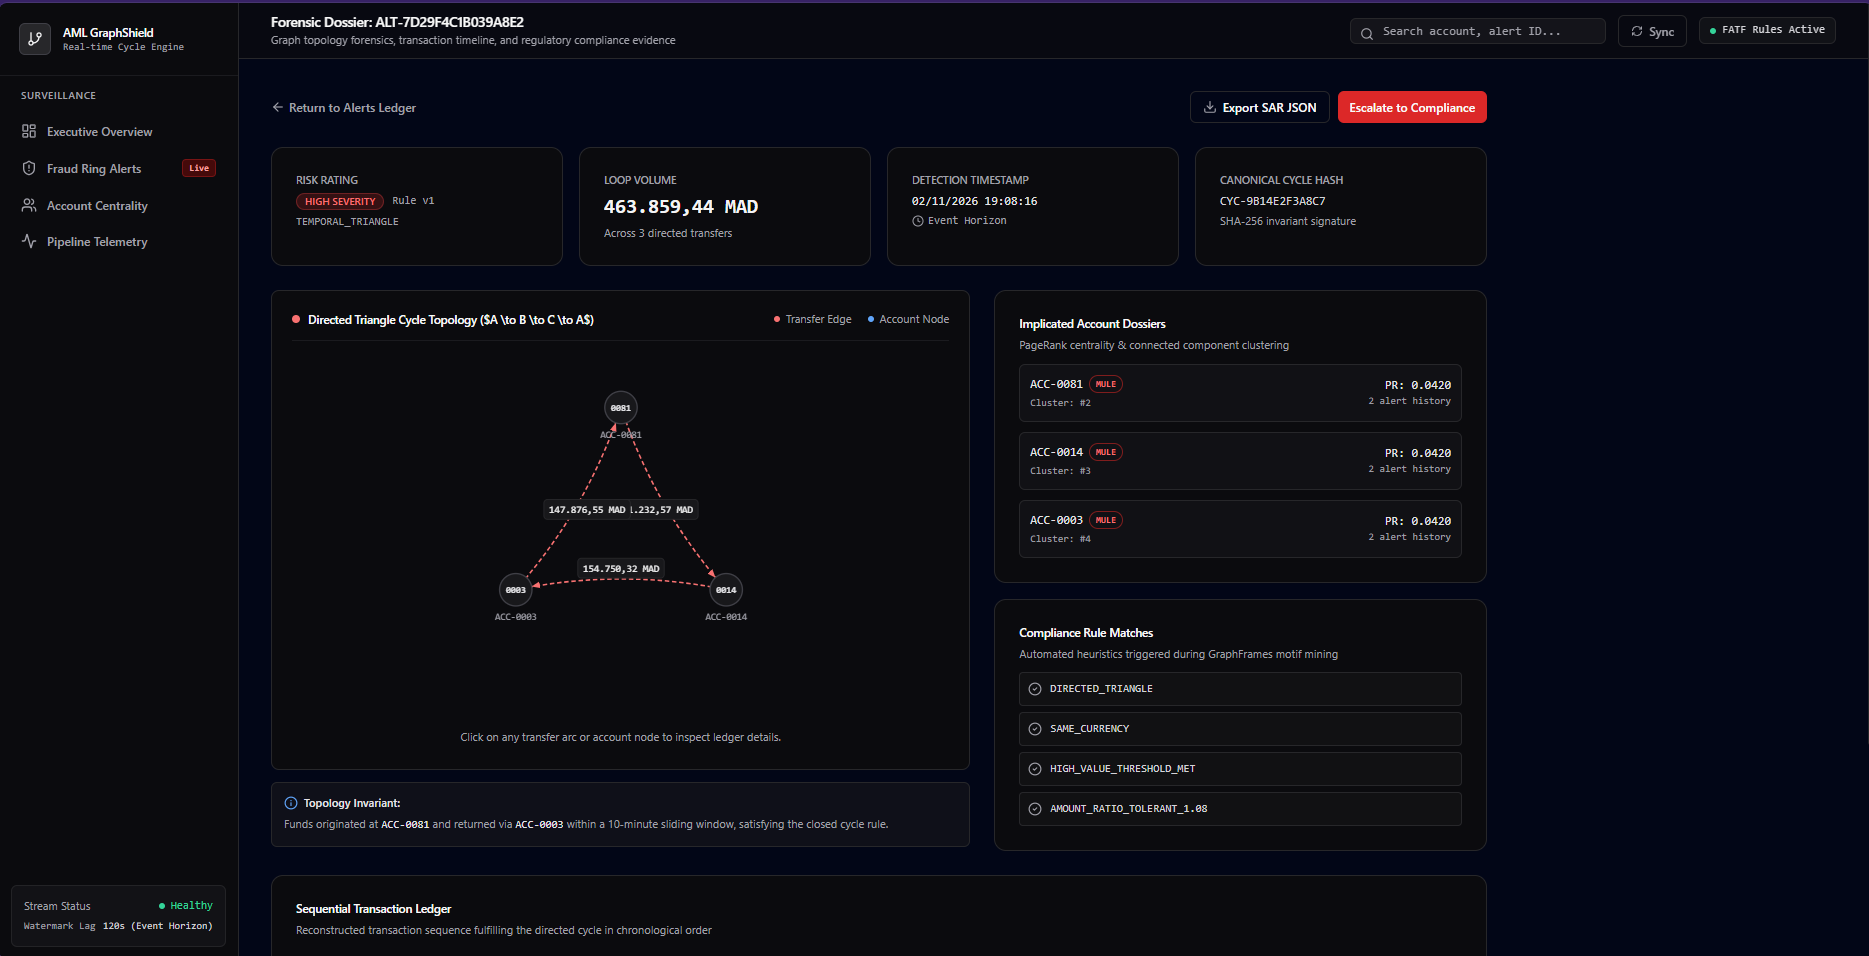
\includegraphics[width=0.92\linewidth]{figures/fig_screenshot_dashboard_graph.png}
    \caption{Composant interactif Directed Canvas Graph : topologie vectorielle d'un cycle fermé ($A \to B \to C \to A$)}
    \label{fig:dash_graph}
\end{figure}

\section{Gestion des dossiers et export réglementaire SAR JSON}

\subsection{Registre des alertes et filtrage dynamique}

La page \texttt{/alerts} (Figure~\ref{fig:dash_cycles}) recense en temps réel l'ensemble des boucles suspectes extraites par le moteur de streaming. L'analyste dispose d'un filtre immédiat par sévérité de risque (\texttt{CRITICAL}, \texttt{HIGH}, \texttt{MEDIUM}) et d'une barre de recherche par identifiant de compte ou de cycle.

\begin{figure}[htbp]
    \centering
    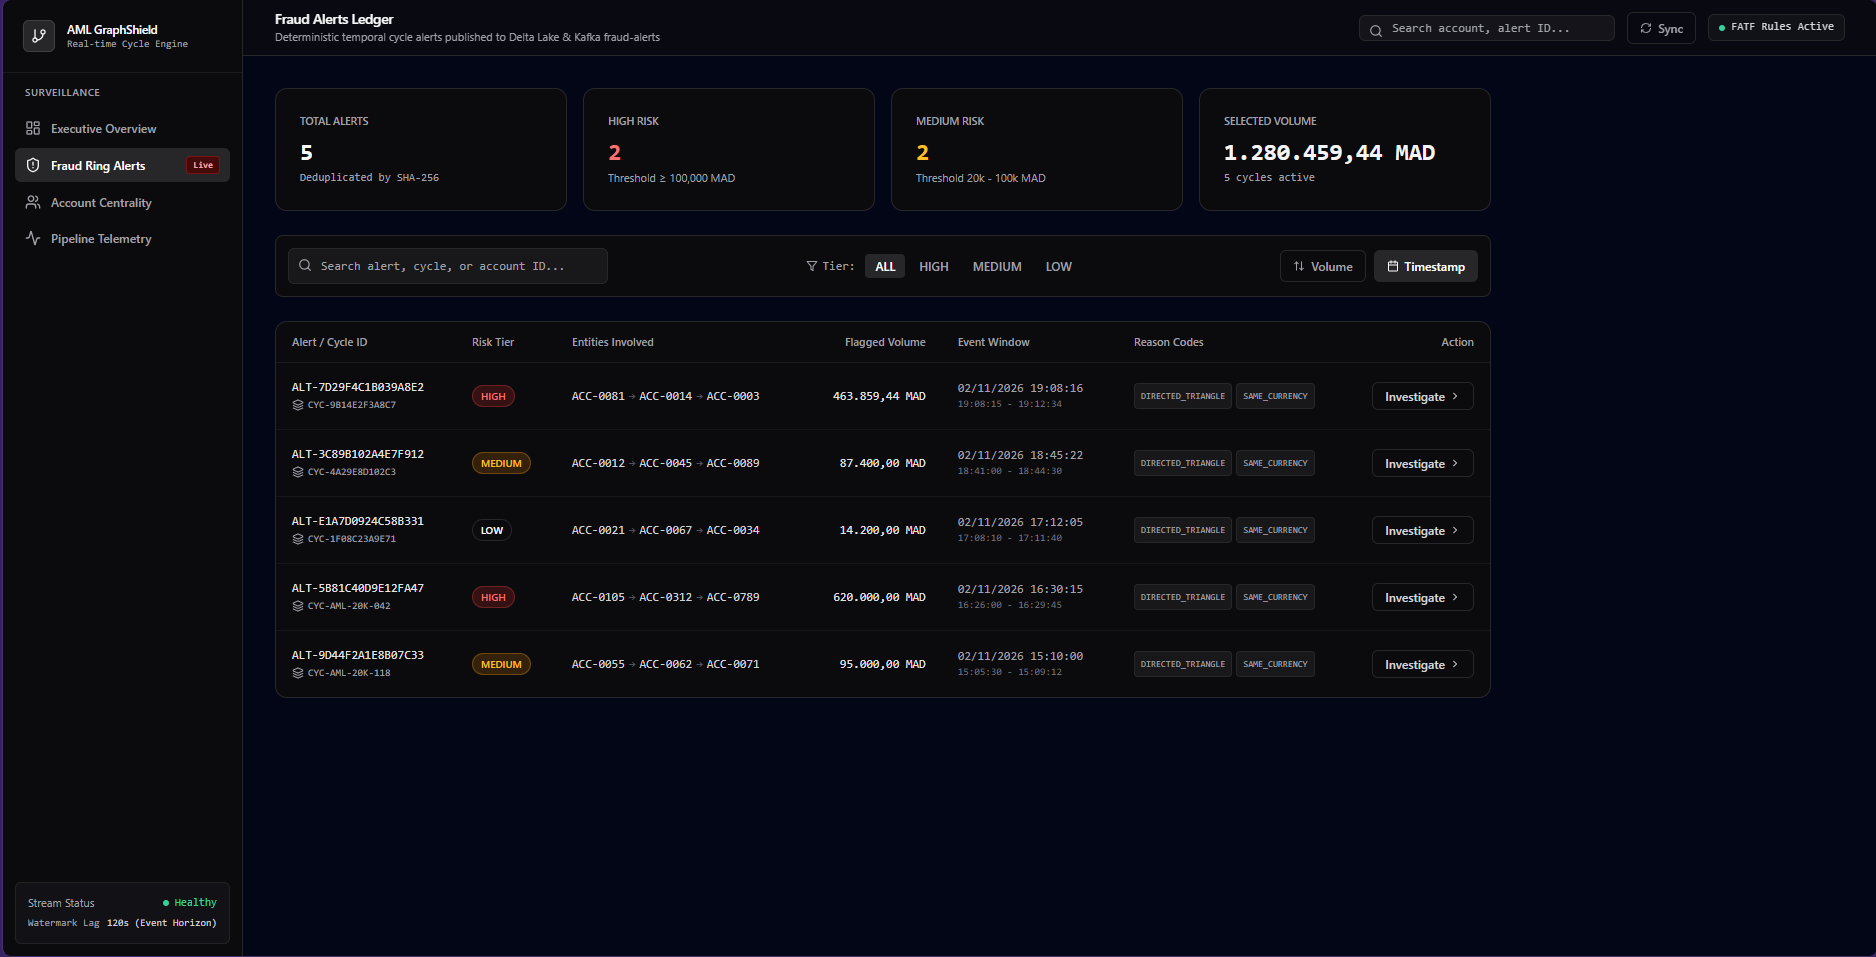
\includegraphics[width=0.92\linewidth]{figures/fig_screenshot_dashboard_cycles.png}
    \caption{Registre médico-légal des alertes de blanchiment et filtrage contextuel par niveau de risque}
    \label{fig:dash_cycles}
\end{figure}

\subsection{Génération automatique de la déclaration de soupçon (SAR JSON)}

Conformément aux normes internationales de conformité bancaire (recommandations du GAFI et directives de l'UTRF), la page d'enquête d'une alerte (\texttt{/investigate/[id]}) intègre un module d'exportation en un clic (Figure~\ref{fig:dash_sar}) générant un dossier officiel de Déclaration de Soupçon (\textit{Suspicious Activity Report} -- SAR) au format JSON standardisé (Listing~\ref{lst:sar_json}) :

\begin{figure}[htbp]
    \centering
    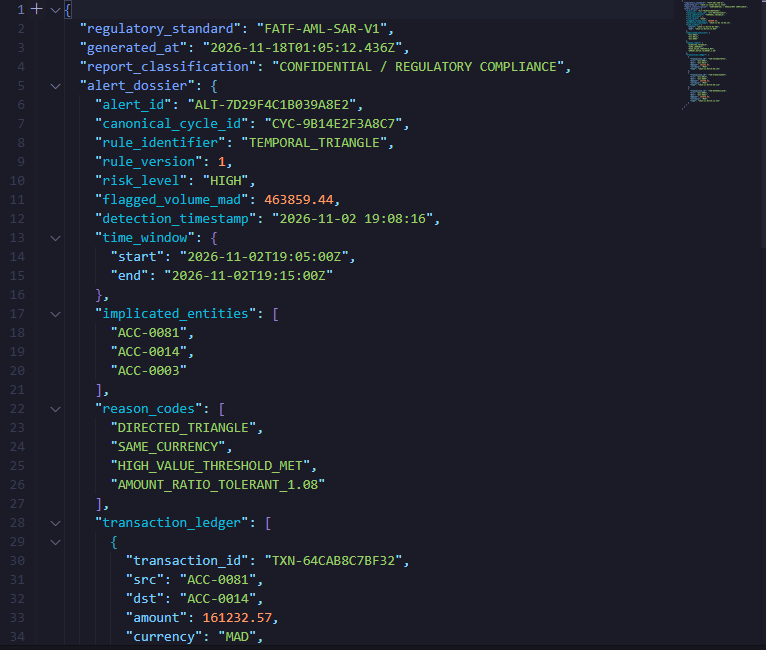
\includegraphics[width=0.68\linewidth]{figures/fig_screenshot_dashboard_sar.png}
    \caption{Boîte de dialogue d'exportation réglementaire SAR (Suspicious Activity Report) au format JSON conforme GAFI/UTRF}
    \label{fig:dash_sar}
\end{figure}

\begin{lstlisting}[language=JSON, caption={Extrait d'un rapport de soupçon (SAR JSON) généré par l'interface}, label={lst:sar_json}]
{
  "sar_report_id": "SAR-20261102-64CAB8",
  "reporting_institution": "AML-GraphShield Engine",
  "filing_timestamp": "2026-11-02T19:35:10Z",
  "alert_metadata": {
    "alert_id": "f8a1c92d4b702e88a3",
    "cycle_id": "a93e110b65f048d08c",
    "risk_level": "CRITICAL",
    "total_laundered_amount": 483697.71,
    "currency": "MAD",
    "duration_seconds": 1845
  },
  "involved_entities": [
    {"account_id": "ACC-0081", "role": "CYCLE_ORIGINATOR", "pagerank": 0.00012},
    {"account_id": "ACC-0014", "role": "INTERMEDIARY_MULE", "pagerank": 0.00009},
    {"account_id": "ACC-0099", "role": "SETTLEMENT_BENEFICIARY", "pagerank": 0.00011}
  ],
  "reason_codes": [
    "CLOSED_CIRCULAR_LOOP_DETECTED",
    "CAPITAL_PRESERVATION_CONFIRMED"
  ]
}
\end{lstlisting}

\section{Console de télémétrie PageRank et monitoring des marchands}

Une vue dédiée (Figure~\ref{fig:dash_pagerank}) permet de consulter la distribution des scores PageRank calculés par Spark et de vérifier en direct que les comptes marchands légitimes sont correctement isolés et ne font l'objet d'aucune fausse alerte (validation visuelle du critère AT-17).

\begin{figure}[htbp]
    \centering
    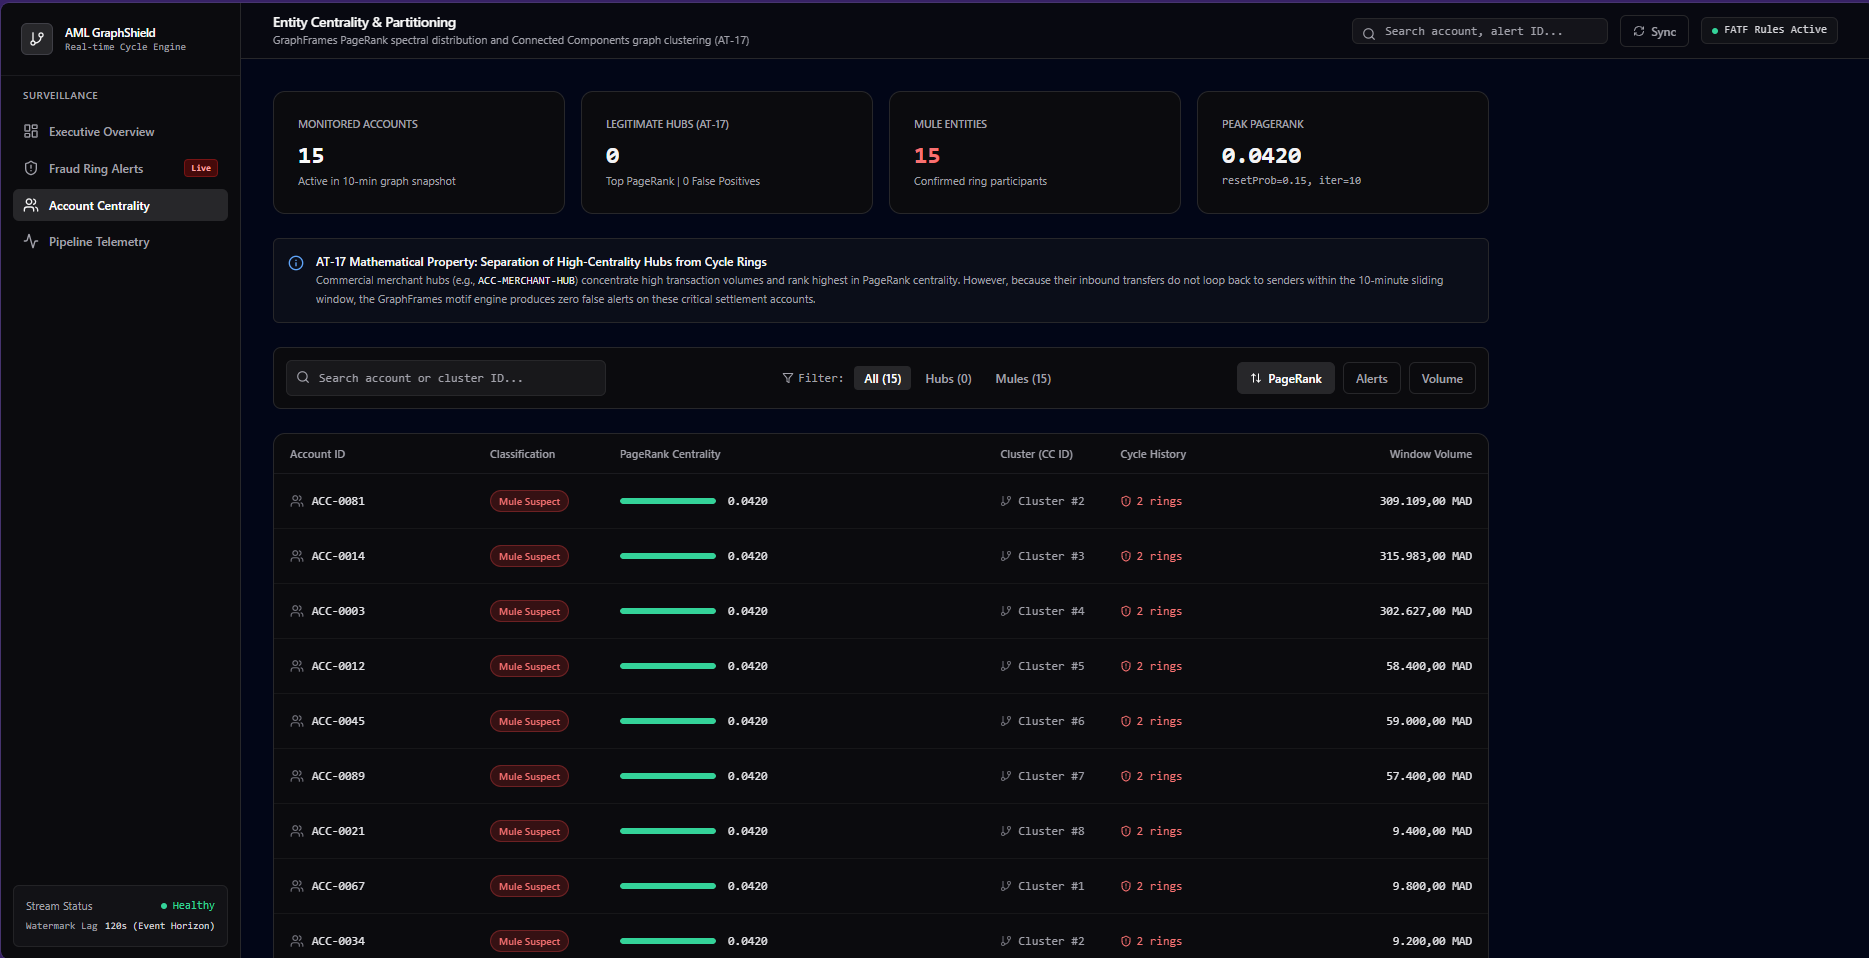
\includegraphics[width=0.92\linewidth]{figures/fig_screenshot_dashboard_pagerank.png}
    \caption{Console de télémétrie PageRank : distribution spectrale des centralités et isolation certifiée des marchands légitimes (AT-17)}
    \label{fig:dash_pagerank}
\end{figure}
